\documentclass[14pt]{beamer}
\usepackage{./Estilos/BeamerUVM}
\usepackage{./Estilos/ColoresLatex}
\usetheme{Madrid}
\usecolortheme{default}
%\useoutertheme{default}
\setbeamercovered{invisible}
% or whatever (possibly just delete it)
\setbeamertemplate{section in toc}[sections numbered]
\setbeamertemplate{subsection in toc}[subsections numbered]
\setbeamertemplate{subsection in toc}{\leavevmode\leftskip=3.2em\rlap{\hskip-2em\inserttocsectionnumber.\inserttocsubsectionnumber}\inserttocsubsection\par}
% \setbeamercolor{section in toc}{fg=blue}
% \setbeamercolor{subsection in toc}{fg=blue}
% \setbeamercolor{frametitle}{fg=blue}
\setbeamertemplate{caption}[numbered]

\setbeamertemplate{footline}
\beamertemplatenavigationsymbolsempty
\setbeamertemplate{headline}{}


\makeatletter
% \setbeamercolor{section in foot}{bg=gray!30, fg=black!90!orange}
% \setbeamercolor{subsection in foot}{bg=blue!30}
% \setbeamercolor{date in foot}{bg=black}
\setbeamertemplate{footline}
{
  \leavevmode%
  \hbox{%
  \begin{beamercolorbox}[wd=.333333\paperwidth,ht=2.25ex,dp=1ex,center]{section in foot}%
    \usebeamerfont{section in foot} {\insertsection}
  \end{beamercolorbox}%
  \begin{beamercolorbox}[wd=.333333\paperwidth,ht=2.25ex,dp=1ex,center]{subsection in foot}%
    \usebeamerfont{subsection in foot}  \insertsubsection
  \end{beamercolorbox}%
  \begin{beamercolorbox}[wd=.333333\paperwidth,ht=2.25ex,dp=1ex,right]{date in head/foot}%
    \usebeamerfont{date in head/foot} \insertshortdate{} \hspace*{2em}
    \insertframenumber{} / \inserttotalframenumber \hspace*{2ex} 
  \end{beamercolorbox}}%
  \vskip0pt%
}
\makeatother

\makeatletter
\patchcmd{\beamer@sectionintoc}{\vskip1.5em}{\vskip0.8em}{}{}
\makeatother

% \usefonttheme{serif}
\usepackage[clock]{ifsym}

\sisetup{per-mode=symbol}
\resetcounteronoverlays{saveenumi}

\title{\Large{Resumen Bloque 2} \\ \normalsize{Física I}}
\date{8 de mayo de 2023}

\begin{document}
\maketitle

\section*{Contenido}
\frame{\frametitle{Contenido} \tableofcontents[currentsection, hideallsubsections]}

\section{M. R. U.}
\frame{\frametitle{Temas revisados} \tableofcontents[currentsection, hideothersubsections]}
\subsection{Conceptos}

\begin{frame}
\frametitle{Conceptos revisados}
\setbeamercolor{item projected}{bg=bananayellow,fg=ao}
\setbeamertemplate{enumerate items}{%
\usebeamercolor[bg]{item projected}%
\raisebox{1.5pt}{\colorbox{bg}{\color{fg}\footnotesize\insertenumlabel}}%
}
\begin{enumerate}[<+->]
\item \textbf{Movimiento}.
\item \textbf{Sistema de referencia}.
\item \textbf{Posición.}
\item \textbf{Desplazamiento}.
\seti
\end{enumerate}
\end{frame}
\begin{frame}
\frametitle{Conceptos revisados}
\setbeamercolor{item projected}{bg=bananayellow,fg=ao}
\setbeamertemplate{enumerate items}{%
\usebeamercolor[bg]{item projected}%
\raisebox{1.5pt}{\colorbox{bg}{\color{fg}\footnotesize\insertenumlabel}}%
}
\begin{enumerate}[<+->]
\conti
\item \textbf{Trayectoria}.
\item \textbf{Velocidad.}
\item \textbf{Aceleración.}
\end{enumerate}
\end{frame}

\subsection{Ecuaciones MRU}

\begin{frame}
\frametitle{Velocidad}
Para calcular la velocidad de un objeto, ocupamos la siguiente expresión:
\pause
\begin{align*}
v = \dfrac{d}{t}
\end{align*}
\end{frame}
\begin{frame}
\frametitle{Representación de utilidad}
En el caso de que un ejercicio nos indique la velocidad, \pause pero nos pida calcular ya sea la \textocolor{red}{distancia} o el \textocolor{ao}{tiempo}, hay que despejar la expresión correspondiente, \pause nos auxiliamos de lo siguiente:
\end{frame}
\begin{frame}
\frametitle{Triángulo de la velocidad}
\begin{figure}
    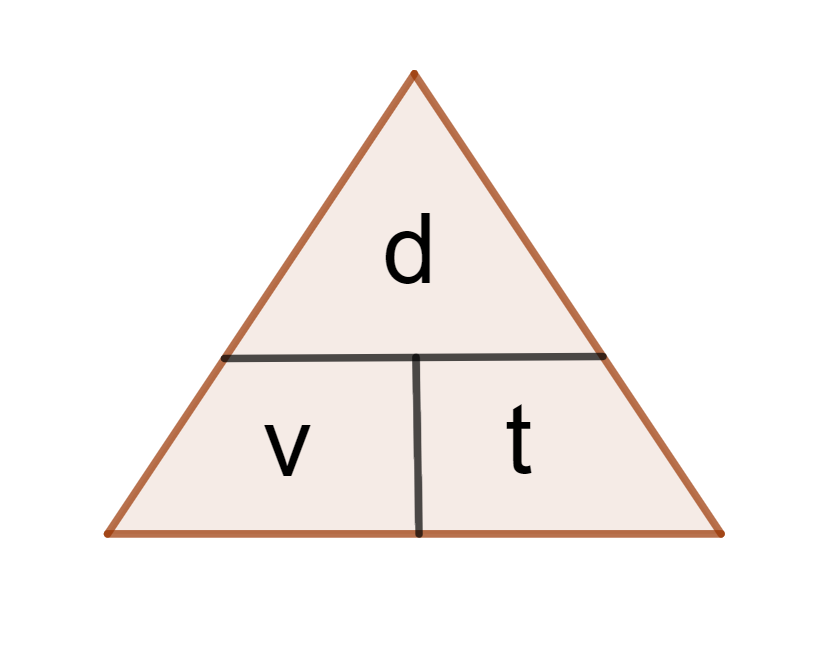
\includegraphics[scale=1]{Imagenes/triangulo_velocidad.png}
\end{figure}
\end{frame}
\begin{frame}
\frametitle{Aceleración}
Calculamos la aceleración con la expresión:
\pause
\begin{align*}
a = \dfrac{v_{f} - v_{i}}{t}
\end{align*}
\end{frame}

\section{M. U. A.}
\frame{\frametitle{Temas revisados} \tableofcontents[currentsection, hideothersubsections]}
\subsection{Aceleración constante}

\begin{frame}
\frametitle{El MUA}
El movimiento uniformemente acelerado (\textocolor{firebrick}{MUA}) es el movimiento que realiza un móvil que varía su velocidad uniformemente, a ese aumento o disminución de la velocidad en cada unidad de tiempo se le conoce como \textocolor{cerise}{aceleración}.
\end{frame}
\begin{frame}
\frametitle{De la aceleración}
\setbeamercolor{item projected}{bg=black,fg=white}
\setbeamertemplate{enumerate items}{%
\usebeamercolor[bg]{item projected}%
\raisebox{1.5pt}{\colorbox{bg}{\color{fg}\footnotesize\insertenumlabel}}%
}
\begin{enumerate}[<+->]
\item Si la velocidad final es mayor que la velocidad inicial entonces la aceleración es positiva y por lo tanto el móvil acelera.
\item Si la velocidad final es menor que la velocidad inicial entonces la aceleración es negativa y por lo tanto el móvil desacelera (frena).
\end{enumerate}
\end{frame}

\subsection{Ecuaciones aceleración constante}

\begin{frame}
\frametitle{Caso con la aceleración constante}
A continuación enlistaremos varias fórmulas que nos permitirán obtener una variable de un objeto que está en movimiento con una \textocolor{carmine}{aceleración constante}.
\end{frame}
\begin{frame}
\frametitle{Ecuaciones de movimiento}
\setbeamercolor{item projected}{bg=firebrick,fg=white}
\setbeamertemplate{enumerate items}{%
\usebeamercolor[bg]{item projected}%
\raisebox{1.5pt}{\colorbox{bg}{\color{fg}\footnotesize\insertenumlabel}}%
}
\begin{enumerate}[<+->]
\item Velocidad como función del tiempo.
\begin{align*}
\setlength{\fboxsep}{3\fboxsep}\boxed{
v_{f} = v_{i} + a \, t
}
\end{align*}
\seti
\end{enumerate}
\end{frame}
\begin{frame}
\frametitle{Ecuaciones de movimiento}
\setbeamercolor{item projected}{bg=firebrick,fg=white}
\setbeamertemplate{enumerate items}{%
\usebeamercolor[bg]{item projected}%
\raisebox{1.5pt}{\colorbox{bg}{\color{fg}\footnotesize\insertenumlabel}}%
}
\begin{enumerate}[<+->]
\conti
\item Posición como función de la velocidad.
\begin{align*}
\setlength{\fboxsep}{3\fboxsep}\boxed{
x_{f} = x_{i} + \dfrac{1}{2} \big( v_{i} + v_{f} \big) \, t
}
\end{align*}
\seti
\end{enumerate}
\end{frame}
\begin{frame}
\frametitle{Ecuaciones de movimiento}
\setbeamercolor{item projected}{bg=firebrick,fg=white}
\setbeamertemplate{enumerate items}{%
\usebeamercolor[bg]{item projected}%
\raisebox{1.5pt}{\colorbox{bg}{\color{fg}\footnotesize\insertenumlabel}}%
}
\begin{enumerate}[<+->]
\conti
\item Posición como función del tiempo.
\begin{align*}
\setlength{\fboxsep}{3\fboxsep}\boxed{
x_{f} = x_{i} + v_{i} \, t + \dfrac{1}{2} a \, t^{2}
}
\end{align*}
\seti
\end{enumerate}
\end{frame}
\begin{frame}
\frametitle{Ecuaciones de movimiento}
\setbeamercolor{item projected}{bg=firebrick,fg=white}
\setbeamertemplate{enumerate items}{%
\usebeamercolor[bg]{item projected}%
\raisebox{1.5pt}{\colorbox{bg}{\color{fg}\footnotesize\insertenumlabel}}%
}
\begin{enumerate}[<+->]
\conti
\item Velocidad como función de la posición
\begin{align*}
\setlength{\fboxsep}{3\fboxsep}\boxed{
v_{f}^{2} = v_{i}^{2} + 2 \, a \big( x_{f} - x_{i}\big)
}
\end{align*}
\end{enumerate}
\end{frame}

\subsection{Caída libre}

\begin{frame}
\frametitle{Influencia de la gravedad}
Un objeto en caída libre es cualquier objeto que se mueve libremente sólo bajo la \textocolor{red}{influencia de la gravedad}, \pause sin importar su movimiento inicial.
\end{frame}
\begin{frame}
\frametitle{Sentido del lanzamiento}
Los objetos que se lanzan hacia arriba o abajo y los que se liberan desde el reposo están todos en caída libre una vez que se liberan.
\end{frame}
\begin{frame}
\frametitle{Sentido del lanzamiento}
Cualquier objeto en caída libre experimenta una aceleración dirigida hacia abajo, sin importar su movimiento inicial.
\end{frame}
\begin{frame}
\frametitle{Escribiendo la aceleración}
La magnitud de la aceleración de caída libre se denota mediante el símbolo $g$.
\\
\bigskip
\pause
El valor de $g$ cerca de la superficie de la Tierra disminuye conforme aumenta la altitud.
\end{frame}
\begin{frame}
\frametitle{El valor de la aceleración}
En la superficie de la Tierra, el valor de $g$ es aproximadamente \SI{9.81}{\meter\per\square\second}.
\end{frame}
\begin{frame}
\frametitle{Expresiones para trabajar}
La \textocolor{carmine}{única modificación} que se necesita hacer en las ecuaciones del M.R.U. para los objetos en caída libre,  es notar que el movimiento es en la dirección vertical (la dirección $y$) \pause antes que en la dirección horizontal $(x)$ \pause y que la aceleración es hacia abajo y tiene una magnitud de \SI{9.81}{\meter\per\square\second}
\end{frame}
\begin{frame}
\frametitle{Sentido de $g$}
En consecuencia, \pause siempre se elegirá:
\pause
\begin{align*}
a = - g = - \SI{9.81}{\meter\per\square\second}
\end{align*}
donde el signo negativo significa que la aceleración de un objeto en caída libre es hacia abajo.
\end{frame}

\section{Reglas en el Examen}
\frame{\tableofcontents[currentsection, hideothersubsections]}
\subsection{Puntos importantes}

\begin{frame}
\frametitle{Para resolver el examen}
Solo necesitarás: bolígrafo, lápiz, goma y una calculadora científica.
\\
\bigskip
\pause
No deberás de utilizar otro objeto sobre la paleta de la banca.
\end{frame}
\begin{frame}
\frametitle{Condiciones de trabajo}
El examen es individual, \pause se deberá de resolver en silencio. \pause Si un alumno o varios, están hablando, se les recogerá el examen, sin discusión.
\\
\bigskip
\pause
En caso de sospecha de usar notas, celular, etc. se recogerá el examen sin discutir el por qué.
\end{frame}

\end{document}